% 由 tools/md2tex.py 自 2020_数学真题_新高考Ⅱ_含解析.md 生成，勿手改（改源 MD 后重跑）


\begin{gknotice}
\textbf{解析归属}：本文档全部解析由本库编写者根据试题独立推导，\textbf{非官方标准答案}。推导过程完整给出以便核验；若与官方发布版本不一致，以官方为准。

\textbf{卷种说明}：2020 年为新高考首批试点年份，本卷（新高考 Ⅱ 卷）由海南使用。
\end{gknotice}

\par\medskip

\gkpart{一、单选题（每小题 5 分，共 40 分）}

\gksolhead{1}{}

\textbf{题目}　设集合 $A=\{2,3,5,7\}$，$B=\{1,2,3,5,8\}$，则 $A\cap B=$（　　）

\textbf{解析}

交集由\textbf{同时属于两个集合}的元素组成。逐个检验 $A$ 中的元素是否也在 $B$ 中：

\begin{center}
\begin{tabular}{ccccc}
\toprule
元素 & $2$ & $3$ & $5$ & $7$ \\
\midrule
是否在 $B$ 中 &  &  &  &  \\
\bottomrule
\end{tabular}
\end{center}

\[A\cap B=\{2,3,5\}\]

\gkanswer{答案：C}

\begin{gktip}
\textbf{易错点}：选项 D 是并集 $A\cup B$ 少了 $7$ 的版本，选项 A 是"只在 $B$ 中"的元素。看清楚是 $\cap$ 还是 $\cup$，这是本题唯一的失分来源。
\end{gktip}

\par\medskip

\gksolhead{2}{}

\textbf{题目}　$(1+2\mathrm i)(2+\mathrm i)=$（　　）

\textbf{解析}

按多项式展开，最后用 $\mathrm i^{2}=-1$ 化简：

\[(1+2\mathrm i)(2+\mathrm i)=1\times2+1\times\mathrm i+2\mathrm i\times2+2\mathrm i\times\mathrm i\]

\[=2+\mathrm i+4\mathrm i+2\mathrm i^{2}=2+5\mathrm i-2=5\mathrm i\]

\gkanswer{答案：B}

\begin{gktip}
\textbf{易错点}：$2\mathrm i^{2}=-2$ 恰好把实部 $2$ 抵消掉，结果是\textbf{纯虚数}。若忘记 $\mathrm i^{2}=-1$ 而当成 $+2$，会得到 $4+5\mathrm i$，四个选项里一个都对不上——这本身就是一个自检信号。
\end{gktip}

\par\medskip

\gksolhead{3}{}

\textbf{题目}　若 $D$ 为 $\triangle ABC$ 的边 $AB$ 的中点，则 $\overrightarrow{CB}=$（　　）

\textbf{解析}

\textbf{中点的向量表达}：$D$ 是 $AB$ 的中点，以 $C$ 为起点写出中线向量

\[\overrightarrow{CD}=\frac12\left(\overrightarrow{CA}+\overrightarrow{CB}\right)\]

（推导：$\overrightarrow{CD}=\overrightarrow{CA}+\overrightarrow{AD}=\overrightarrow{CA}+\dfrac12\overrightarrow{AB}=\overrightarrow{CA}+\dfrac12\left(\overrightarrow{CB}-\overrightarrow{CA}\right)=\dfrac12\left(\overrightarrow{CA}+\overrightarrow{CB}\right)$。）

两边乘 $2$ 后移项，解出 $\overrightarrow{CB}$：

\[2\overrightarrow{CD}=\overrightarrow{CA}+\overrightarrow{CB}\ \Longrightarrow\ \overrightarrow{CB}=2\overrightarrow{CD}-\overrightarrow{CA}\]

\textbf{坐标验证}：取 $C(0,0)$、$A(1,0)$、$B(0,1)$，则 $D\left(\dfrac12,\dfrac12\right)$。

\[2\overrightarrow{CD}-\overrightarrow{CA}=2\left(\frac12,\frac12\right)-(1,0)=(1,1)-(1,0)=(0,1)=\overrightarrow{CB}\quad\checkmark\]

顺带排除其余三项：$2\overrightarrow{CA}-\overrightarrow{CD}=\left(\dfrac32,-\dfrac12\right)$，$2\overrightarrow{CD}+\overrightarrow{CA}=(2,1)$，$2\overrightarrow{CA}+\overrightarrow{CD}=\left(\dfrac52,\dfrac12\right)$，均不等于 $(0,1)$。

\gkanswer{答案：A}

\begin{gktip}
\textbf{方法总结}：向量选择题若一时看不出变形方向，\textbf{直接取一组具体坐标代入验证}是最快的路线——四个选项一次性全部判定，且不会因为符号写反而失分。中点公式 $\overrightarrow{CD}=\dfrac12\left(\overrightarrow{CA}+\overrightarrow{CB}\right)$ 本身必须背熟，它是"三角形中线"类问题的起点。
\end{gktip}

\par\medskip

\gksolhead{4}{}

\textbf{题目}　日晷是中国古代用来测定时间的仪器，利用与晷面垂直的晷针投射到晷面的影子来测定时间。把地球看成一个球（球心记为 $O$），地球上一点 $A$ 的纬度是指 $OA$ 与地球赤道所在平面所成角，点 $A$ 处的水平面是指过点 $A$ 且与 $OA$ 垂直的平面。在点 $A$ 处放置一个日晷，若晷面与赤道所在平面平行，点 $A$ 处的纬度为北纬 $40^\circ$，则晷针与点 $A$ 处的水平面所成角为（　　）

\textbf{解析}

\textbf{第一步，弄清晷针的方向。}

\begin{itemize}
\item 晷针 $\perp$ 晷面（题设）；
\item 晷面 $\parallel$ 赤道面（题设）。
\end{itemize}

由"垂直于两平行平面之一必垂直于另一个"，得

\[\text{晷针}\perp\text{赤道面}\]

即\textbf{晷针与地轴平行}（地轴正是垂直于赤道面的那条直线）。

\textbf{第二步，把两个角联系起来。}

设地轴方向为 $\boldsymbol n$。纬度的定义给出 $OA$ 与赤道面所成角为 $40^\circ$，而 $\boldsymbol n\perp$ 赤道面，故 $OA$ 与 $\boldsymbol n$ 的夹角为

\[90^\circ-40^\circ=50^\circ\]

\textbf{第三步，用"线面角 = 余角"完成转化。}

点 $A$ 处的水平面 $\perp OA$，也就是说 \textbf{$OA$ 是水平面的法方向}。

直线与平面所成的角，等于 $90^\circ$ 减去该直线与平面法线的夹角：

\[\text{晷针与水平面所成角}=90^\circ-\underbrace{50^\circ}_{\text{晷针}(\parallel\boldsymbol n)\text{ 与 }OA\text{ 的夹角}}=40^\circ\]

\gkanswer{答案：B}

\begin{gktip}
\textbf{一般结论}（值得记住）：\textbf{晷针与当地水平面所成角恰好等于当地纬度}。这正是日晷安装的通用规则——晷针指向北天极，其仰角就是安装地的纬度。本题把这条常识用"两次取余角"严格证明了一遍。

\textbf{易错点}：选项 C 的 $50^\circ$ 是"晷针与 $OA$ 的夹角"，是中间量而不是答案。做立体几何的角度题，\textbf{每算出一个角都要问一句"这是我要的那个角吗"}。
\end{gktip}

\par\medskip

\gksolhead{5}{}

\textbf{题目}　某中学的学生积极参加体育锻炼，其中有 $96\%$ 的学生喜欢足球或游泳，$60\%$ 的学生喜欢足球，$82\%$ 的学生喜欢游泳，则该中学既喜欢足球又喜欢游泳的学生数占该校学生总数的比例是（　　）

\textbf{解析}

记 $P$ 为喜欢足球的比例、$Q$ 为喜欢游泳的比例。\textbf{容斥原理}（两集合的并）：

\[|P\cup Q|=|P|+|Q|-|P\cap Q|\]

代入题给数据：

\[96\%=60\%+82\%-|P\cap Q|\]

\[|P\cap Q|=60\%+82\%-96\%=46\%\]

\gkanswer{答案：C}

\begin{gktip}
\textbf{方法总结}：$60\%+82\%=142\%>100\%$，超出的 $42\%$ 说明必有重叠。注意重叠部分不是 $42\%$（那是"假设人人至少喜欢一项"时的答案，对应干扰项 D）——真正的重叠是 $142\%-96\%=46\%$，因为还有 $4\%$ 的学生两项都不喜欢。\textbf{先算出"两项都不喜欢"的比例（$4\%$）再验算，是本题最好的自检手段。}
\end{gktip}

\par\medskip

\gksolhead{6}{}

\textbf{题目}　$3$ 名大学生利用假期到 $2$ 个山村参加扶贫工作，每名大学生只去 $1$ 个村，每个村至少 $1$ 人，则不同的分配方案共有（　　）

\textbf{解析}

\textbf{方法一（正难则反，最快）}

每名大学生各有 $2$ 种选择，不加限制时共

\[2^{3}=8\ \text{种}\]

其中不合要求的只有"$3$ 人全去甲村"和"$3$ 人全去乙村"两种（会使另一村无人）。故

\[8-2=6\ \text{种}\]

\textbf{方法二（先分组再分配）}

每村至少 $1$ 人且共 $3$ 人，人数只能按 $2+1$ 分配。

\begin{itemize}
\item 先把 $3$ 人分成一个 $2$ 人组和一个 $1$ 人组：$\mathrm C_3^{1}=3$ 种（选出单独的那一人即可）；
\item 再把两组分配到两个村（村是有区别的）：$\mathrm A_2^{2}=2$ 种。
\end{itemize}

\[3\times2=6\ \text{种}\]

\gkanswer{答案：C}

\begin{gktip}
\textbf{易错点}：选项 D 的 $8$ 正是漏掉"每村至少 $1$ 人"限制的结果；选项 A 的 $4$ 则是把两个村当成无区别的（只数分组不数分配）。\textbf{两个村是不同的地点，分组之后必须再乘以分配的顺序数。}
\end{gktip}

\par\medskip

\gksolhead{7}{}

\textbf{题目}　已知函数 $f(x)=\lg\left(x^{2}-4x-5\right)$ 在 $(a,+\infty)$ 单调递增，则 $a$ 的取值范围是（　　）

\textbf{解析}

\textbf{第一步（必须先做）：求定义域。}

\[x^{2}-4x-5>0\ \Longleftrightarrow\ (x-5)(x+1)>0\ \Longleftrightarrow\ x<-1\ \text{或}\ x>5\]

定义域为 $(-\infty,-1)\cup(5,+\infty)$。

\textbf{第二步，分析复合函数的单调性。}

外层 $y=\lg u$ 在 $u>0$ 上\textbf{递增}，故 $f$ 的单调性与内层 $u=x^{2}-4x-5$ 一致（"同增异减"）。

内层是开口向上、对称轴 $x=2$ 的抛物线：在 $(-\infty,2)$ 递减、在 $(2,+\infty)$ 递增。

与定义域取交：

\begin{center}
\begin{tabular}{ccc}
\toprule
区间 & $(-\infty,-1)$ & $(5,+\infty)$ \\
\midrule
内层 $u$ & 递减（在对称轴左侧） & 递增（在对称轴右侧） \\
$f$ & 递减 & \textbf{递增} \\
\bottomrule
\end{tabular}
\end{center}

所以 $f$ 的\textbf{唯一}单调递增区间是 $(5,+\infty)$。

\textbf{第三步，翻译题目要求。}

"$f$ 在 $(a,+\infty)$ 单调递增"要求 $(a,+\infty)$ 是递增区间的\textbf{子集}：

\[(a,+\infty)\subseteq(5,+\infty)\ \Longleftrightarrow\ a\ge5\]

\gkanswer{答案：D}

\begin{gktip}
\textbf{易错点}（本题最大的坑）：只盯着内层抛物线"在 $x>2$ 递增"而选 C 的 $[2,+\infty)$——但 $x\in(2,5]$ 时根本\textbf{不在定义域内}（对数的真数 $\le0$），函数在那里没有定义，谈不上单调。

\textbf{通用纪律}：\textbf{含对数、根式、分式的单调性问题，第一步永远是求定义域}，第二步才谈单调性，最后取交集。顺序反了就会掉进 C。
\end{gktip}

\par\medskip

\gksolhead{8}{}

\textbf{题目}　若定义在 $\mathbf R$ 的奇函数 $f(x)$ 在 $(-\infty,0)$ 单调递减，且 $f(2)=0$，则满足 $xf(x-1)\ge0$ 的 $x$ 的取值范围是（　　）

\textbf{解析}

\textbf{第一步，把 $f$ 的符号表补全。}

\begin{itemize}
\item $f$ 是\textbf{奇函数}，且在 $(-\infty,0)$ 递减 → 在 $(0,+\infty)$ 也\textbf{递减}（奇函数在关于原点对称的两个区间上单调性相同）；
\item $f(2)=0$，由奇性得 $f(-2)=-f(2)=0$；
\item $f$ 定义在 $\mathbf R$ 上且为奇函数 → $f(0)=0$。
\end{itemize}

在 $(0,+\infty)$ 上 $f$ 递减且 $f(2)=0$：$0<x<2$ 时 $f>0$，$x>2$ 时 $f<0$。再由奇性翻到左边：

\begin{center}
\begin{tabular}{cccccccc}
\toprule
$x$ & $(-\infty,-2)$ & $-2$ & $(-2,0)$ & $0$ & $(0,2)$ & $2$ & $(2,+\infty)$ \\
\midrule
$f(x)$ 的符号 & $+$ & $0$ & $-$ & $0$ & $+$ & $0$ & $-$ \\
\bottomrule
\end{tabular}
\end{center}

于是

\[f(t)\ge0\ \Longleftrightarrow\ t\le-2\ \text{或}\ 0\le t\le2\]
\[f(t)\le0\ \Longleftrightarrow\ -2\le t\le0\ \text{或}\ t\ge2\]

\textbf{第二步，按 $x$ 的符号分三种情形解 $xf(x-1)\ge0$。}

\textbf{情形一：$x>0$。} 需 $f(x-1)\ge0$：

\[x-1\le-2\ \text{或}\ 0\le x-1\le2\ \Longrightarrow\ x\le-1\ \text{或}\ 1\le x\le3\]

与 $x>0$ 取交：$1\le x\le3$。

\textbf{情形二：$x=0$。} 此时 $xf(x-1)=0\ge0$ 成立，$x=0$ \textbf{是解}。

\textbf{情形三：$x<0$。} 需 $f(x-1)\le0$：

\[-2\le x-1\le0\ \text{或}\ x-1\ge2\ \Longrightarrow\ -1\le x\le1\ \text{或}\ x\ge3\]

与 $x<0$ 取交：$-1\le x<0$。

\textbf{第三步，合并。}

\[[-1,0)\cup\{0\}\cup[1,3]=[-1,0]\cup[1,3]\]

\gkanswer{答案：D}

\begin{gktip}
\textbf{易错点}：
① \textbf{$x=0$ 必须单独讨论}——它使乘积为 $0$，满足"$\ge0$"。漏掉它会把答案写成 $[-1,0)\cup[1,3]$，与四个选项都对不上。
② 选项 C 的 $[1,+\infty)$ 忽略了 $x>3$ 时 $f(x-1)<0$（因为 $x-1>2$）；选项 A 把 $[3,+\infty)$ 当成解，正是这个错误的另一种写法。
③ \textbf{"奇函数在两侧单调性相同、偶函数在两侧单调性相反"}——这条必须条件反射，否则第一步的符号表就是错的。
\end{gktip}

\par\medskip

\gkpart{二、多选题（每小题 5 分，共 20 分）}

\gksolhead{9}{}

\textbf{题目}　我国新冠肺炎疫情进入常态化，各地有序推进复工复产，下面是某地连续 $11$ 天复工复产指数折线图，下列说法正确的是（　　）

\begin{center}% 2020 新高考Ⅱ卷 9：某地区复工复产指数折线图（连续 11 天）
% 绘制依据：源 PDF 原图逐点核对。横轴「天数」等距标 1–11；纵轴「指数」不从 0 起，
% 只画 78%/80%/82% 三条水平虚线并在左侧标注；右上角图例：空心圆＝复产指数，实心圆＝复工指数。
% 必须保住的形态：第 2 天复工为全图最低且恰在 78% 线上；第 6 天复工恰在 82% 线上；
% 第 3 天起两线均在 80% 线上方；第 8→9 天两线交叉，其后复工在上（第 11 天复产重新略高）；
% 第 1 天两线间距明显大于第 11 天。
% 说明：第 2 天复工取 78.0、第 6 天复工取 82.0（转录读数 77.9 / 82.1），
% 以保住原图「恰落在虚线上」的定性特征——0.1 的差在本图尺度上会明显浮出虚线。
\begin{tikzpicture}
\begin{axis}[width=10.6cm, height=6.4cm, font=\small,
  axis lines=left,
  xlabel={天数}, ylabel={指数},
  xlabel style={at={(1,0)}, anchor=north west},
  ylabel style={at={(0,1)}, anchor=south, rotate=-90},
  xmin=0.35, xmax=11.75, ymin=76.9, ymax=87.4,
  xtick={1,2,...,11},
  ytick={78,80,82},
  yticklabels={$78\%$,$80\%$,$82\%$},
  ymajorgrids=true, grid style={dashed, gray!65},
  legend cell align=left,
  legend style={at={(0.995,0.99)}, anchor=north east, draw=none, fill=white,
                font=\small, row sep=-2pt, inner sep=2pt}]
  \addplot[thick, mark=o, mark size=1.7pt, mark options={fill=white}]
    coordinates {(1,80.6) (2,80.8) (3,81.6) (4,82.4) (5,82.6) (6,83.0)
                 (7,84.0) (8,83.4) (9,81.6) (10,82.8) (11,84.4)};
  \addlegendentry{复产指数}
  \addplot[thick, mark=*, mark size=1.7pt]
    coordinates {(1,79.7) (2,78.0) (3,80.5) (4,81.1) (5,81.3) (6,82.0)
                 (7,82.3) (8,81.7) (9,83.2) (10,84.5) (11,83.9)};
  \addlegendentry{复工指数}
\end{axis}
\end{tikzpicture}
\end{center}

\textbf{解析}

先按图读出两条折线的近似数值（读数精确到 $0.1$ 个百分点，用于定量核对；判断时以图形的相对高低为准）：

\begin{center}
\begin{tabular}{cccccccccccc}
\toprule
天数 & $1$ & $2$ & $3$ & $4$ & $5$ & $6$ & $7$ & $8$ & $9$ & $10$ & $11$ \\
\midrule
复工（实心） & $79.7$ & $77.9$ & $80.5$ & $81.1$ & $81.3$ & $82.1$ & $82.3$ & $81.7$ & $83.2$ & $84.5$ & $83.9$ \\
复产（空心） & $80.6$ & $80.8$ & $81.6$ & $82.4$ & $82.6$ & $83.0$ & $84.0$ & $83.4$ & $81.6$ & $82.8$ & $84.4$ \\
\bottomrule
\end{tabular}
\end{center}

\par\medskip

\textbf{A （"均逐日增加"）}

只要找到\textbf{一处下降}即可否定。第 $1$ 天到第 $2$ 天，复工指数明显\textbf{下降}（图中第 $2$ 天的实心点落到最低的 $78\%$ 虚线上）。

此外复产指数在第 $7\to8$ 天、第 $8\to9$ 天也在下降。A 错。

\par\medskip

\textbf{B （整段 $11$ 天，复产增量 > 复工增量）}

"增量"指\textbf{末值减初值}，与中间过程无关。

\textbf{不依赖精确读数的判法}：第 $1$ 天复产指数\textbf{明显高于}复工指数（约差 $0.9$ 个百分点）；到第 $11$ 天，复产虽仍略高，但两点已经贴得很近（约差 $0.5$ 个百分点）。\textbf{两条线的差距在缩小，说明这 $11$ 天里复工指数涨得更多。}

定量核对：

\[\text{复工增量}\approx83.9-79.7=4.2,\qquad \text{复产增量}\approx84.4-80.6=3.8\]

复工增量更大，B 错。

\par\medskip

\textbf{C （第 $3$ 天至第 $11$ 天两指数均超过 $80\%$）}

从第 $3$ 天起，两条折线的所有数据点都落在 $80\%$ 虚线\textbf{上方}（复工在第 $3$ 天恰好刚越过 $80\%$，是这九天里最低的一点，约 $80.5\%$）。C 对。

\par\medskip

\textbf{D （第 $9$ 天至第 $11$ 天，复产增量 > 复工增量）}

第 $8$ 天到第 $9$ 天两条线\textbf{发生交叉}：复工指数跃升并反超，复产指数回落到 $82\%$ 虚线之下。因此第 $9$ 天是复产的一个\textbf{低谷}、却是复工的一个\textbf{高位}，此后两天：

\[\text{复产增量}\approx84.4-81.6=2.8,\qquad \text{复工增量}\approx83.9-83.2=0.7\]

复产增量更大，D 对。

\gkanswer{答案：CD}

\begin{gktip}
\textbf{方法总结}：B 与 D 用的是\textbf{同一个判据}（末值减初值），结论却相反——差别只在于\textbf{区间端点选在哪里}。这正是命题人的设计：考生若把"复产整体位置更高"误当成"复产涨得更多"，就会把 B 判对。

\textbf{读图题的三条纪律}：① "均/都"类命题只需\textbf{一个反例}即可否定（A）；② "增量"只看\textbf{两个端点}，不看中间起伏（B、D）；③ 涉及"超过某条虚线"时，找出该区间内\textbf{最低的那个点}去比（C）。
\end{gktip}

\par\medskip

\gksolhead{10}{}

\textbf{题目}　已知曲线 $C:mx^{2}+ny^{2}=1$（　　）

\textbf{解析}

把方程化成标准形式（当 $m,n$ 均不为 $0$ 时）：

\[\frac{x^{2}}{\dfrac1m}+\frac{y^{2}}{\dfrac1n}=1\]

\par\medskip

\textbf{A （$m>n>0$ 时是焦点在 $y$ 轴上的椭圆）}

$m,n>0$ 时两个分母 $\dfrac1m,\dfrac1n$ 均为正，曲线是椭圆。

由 $m>n>0$ 得

\[\frac1m<\frac1n\]

即 $y^{2}$ 下面的分母\textbf{更大}，长轴沿 $y$ 轴，\textbf{焦点在 $y$ 轴上} 

\par\medskip

\textbf{B （$m=n>0$ 时半径不是 $\sqrt n$）}

$m=n>0$ 时方程为 $n\left(x^{2}+y^{2}\right)=1$，即

\[x^{2}+y^{2}=\frac1n\]

这是圆，但半径为

\[r=\sqrt{\frac1n}=\frac{\sqrt n}n\ne\sqrt n\qquad(n\ne1)\]

例如 $n=4$ 时真实半径是 $\dfrac12$，而选项声称 $2$。B 错。

\par\medskip

\textbf{C （$mn<0$ 时是双曲线，渐近线 $y=\pm\sqrt{-\dfrac mn}\,x$）}

$mn<0$ 说明 $\dfrac1m$ 与 $\dfrac1n$ 异号，方程为双曲线 

\textbf{渐近线}由方程的"$1$ 换成 $0$"得到：

\[mx^{2}+ny^{2}=0\ \Longrightarrow\ y^{2}=-\frac mn x^{2}\]

因 $mn<0$ 有 $-\dfrac mn>0$，可以开方：

\[y=\pm\sqrt{-\frac mn}\,x\quad\checkmark\]

\par\medskip

\textbf{D （$m=0$，$n>0$ 时是两条直线）}

$m=0$ 时方程退化为

\[ny^{2}=1\ \Longrightarrow\ y^{2}=\frac1n\ \Longrightarrow\ y=\pm\frac1{\sqrt n}\]

这是两条平行于 $x$ 轴的直线 

\gkanswer{答案：ACD}

\begin{gktip}
\textbf{方法总结}：这类"含参二次曲线判型"题的标准动作是\textbf{先化标准形（把 $1$ 挪到右边、系数变成分母）}，再按分母的正负与大小判断类型和焦点位置。

\textbf{B 项的陷阱极其典型}：$x^{2}+y^{2}=\dfrac1n$ 的半径是 $\sqrt{\dfrac1n}$ 而不是 $\sqrt n$。\textbf{看到"半径为 $\sqrt{\text{\text{系数}}}$"这种说法，一定要回头核对是系数本身还是系数的倒数。}

\textbf{渐近线的求法}（值得背）：双曲线 $\dfrac{x^{2}}{A}-\dfrac{y^{2}}{B}=1$ 的渐近线就是把右边的 $1$ 换成 $0$ 后分解出来的两条直线。这个方法对本题这种"没化成标准形"的方程同样直接可用。
\end{gktip}

\par\medskip

\gksolhead{11}{}

\textbf{题目}　下图是函数 $y=\sin(\omega x+\varphi)$ 的部分图象，则 $\sin(\omega x+\varphi)=$（　　）

\begin{center}% 2020 新高考Ⅱ卷 11：正弦型函数 y=sin(2x+2π/3) 的图象，x∈[−π/3, 7π/6]
% 绘制依据：源 PDF 原图。形态锚点：最大值在 x=−π/12（y 轴稍左）、x=π/6 处下穿 x 轴、
% 最小值 x=5π/12、x=2π/3 处上穿、x=11π/12 再现波峰；区间两端恰为零点（跨 1.5 个周期）。
% y 轴只标刻度 1（置于 (0,1) 左上方以避开紧邻 y 轴的波峰）；
% x 轴只标 π/6 与 2π/3，用手工节点分置左下 / 右下以避让曲线；O 标原点左下。
\begin{tikzpicture}
\begin{axis}[width=10.6cm, height=5.6cm, font=\small,
  axis lines=middle, xlabel={$x$}, ylabel={$y$},
  xmin=-1.35, xmax=4.05, ymin=-1.45, ymax=1.62,
  xtick=\empty, ytick=\empty,
  every axis x label/.style={at={(current axis.right of origin)}, anchor=west},
  every axis y label/.style={at={(current axis.above origin)}, anchor=south}]
  \addplot[domain=-1.0472:3.6652, samples=250, thick] {sin(deg(2*x+2*pi/3))};
  \draw (axis cs:-0.06,1) -- (axis cs:0.06,1);
  \node[above left, inner sep=1pt] at (axis cs:0,1) {$1$};
  \node[below left, inner sep=1pt] at (axis cs:0.5236,0) {$\frac{\pi}{6}$};
  \node[below right, inner sep=1pt] at (axis cs:2.0944,0) {$\frac{2\pi}{3}$};
  \node[below left, inner sep=1pt] at (axis cs:0,0) {$O$};
\end{axis}
\end{tikzpicture}
\end{center}

\textbf{解析}

\textbf{第一步，从图上读出三条关键信息。}

1. $x=\dfrac\pi6$ 是一个\textbf{下降零点}（曲线由正变负）；
2. $x=\dfrac{2\pi}3$ 是一个\textbf{上升零点}（曲线由负变正）；
3. 最大值 $1$ 在 $y$ 轴\textbf{稍左侧}取到，因此 $f(0)$ 略小于 $1$（是正数）。

\textbf{第二步，由两个相邻零点定 $\omega$。}

相邻两个零点相差\textbf{半个周期}：

\[\frac T2=\frac{2\pi}3-\frac\pi6=\frac{4\pi-\pi}6=\frac\pi2\ \Longrightarrow\ T=\pi\ \Longrightarrow\ \omega=\frac{2\pi}T=2\]

\textbf{第三步，由下降零点定 $\varphi$。}

$\sin$ 的下降零点满足"相位 $=\pi+2k\pi$"：

\[2\times\frac\pi6+\varphi=\pi+2k\pi\ \Longrightarrow\ \varphi=\frac{2\pi}3+2k\pi\]

取 $k=0$：

\[y=\sin\left(2x+\frac{2\pi}3\right)\]

\textbf{校验}：$f(0)=\sin\dfrac{2\pi}3=\dfrac{\sqrt3}2\approx0.87$，确实是略小于 $1$ 的正数；最大值点由 $2x+\dfrac{2\pi}3=\dfrac\pi2$ 得 $x=-\dfrac\pi{12}<0$，在 $y$ 轴左侧 

\textbf{第四步，把四个选项统一化成 $\sin(2x+\cdot)$ 的形式逐项比对。}

\textbf{A} $\sin\left(x+\dfrac\pi3\right)$：$\omega=1$，周期 $2\pi$，与图象周期 $\pi$ 不符。且 $f\left(\dfrac\pi6\right)=\sin\dfrac\pi2=1\ne0$ 

\textbf{B} $\sin\left(\dfrac\pi3-2x\right)$：用 $\sin\theta=\sin(\pi-\theta)$：

\[\sin\left(\frac\pi3-2x\right)=\sin\left[\pi-\left(\frac\pi3-2x\right)\right]=\sin\left(2x+\frac{2\pi}3\right)\quad\checkmark\]

\textbf{C} $\cos\left(2x+\dfrac\pi6\right)$：用 $\cos\theta=\sin\left(\dfrac\pi2-\theta\right)$：

\[\cos\left(2x+\frac\pi6\right)=\sin\left(\frac\pi2-2x-\frac\pi6\right)=\sin\left(\frac\pi3-2x\right)\]

\textbf{这与 B 是同一个函数}，故也等于 $\sin\left(2x+\dfrac{2\pi}3\right)$ 

\textbf{D} $\cos\left(\dfrac{5\pi}6-2x\right)$：

\[\cos\left(\frac{5\pi}6-2x\right)=\sin\left(\frac\pi2-\frac{5\pi}6+2x\right)=\sin\left(2x-\frac\pi3\right)\]

在 $x=\dfrac\pi6$ 处：$\sin0=0$ 确为零点，但它是\textbf{上升}零点（导数 $2\cos0=2>0$），与图象在此处下降相矛盾；且 $f(0)=\sin\left(-\dfrac\pi3\right)=-\dfrac{\sqrt3}2<0$，与图象在 $y$ 轴附近取正值矛盾 

\gkanswer{答案：BC}

\begin{gktip}
\textbf{关键洞察}：\textbf{B 与 C 是同一个函数的两种写法}，因此必须\textbf{同时选}。多选题中出现"两个选项恒等"的情形并不常见，一旦发现，就说明它们要么全对、要么全错——这本身就是一个强有力的验算手段。

\textbf{D 与 B 只差一个符号}（$\sin\left(2x-\dfrac\pi3\right)$ 与 $\sin\left(2x+\dfrac{2\pi}3\right)$ 恰好互为相反数），是本题最大的干扰项。\textbf{区分它们只需一个信息：$x=\dfrac\pi6$ 处曲线是往下穿还是往上穿。} 只核对"是不是零点"会同时放过 B、C、D 三项。
\end{gktip}

\par\medskip

\gksolhead{12}{}

\textbf{题目}　已知 $a>0$，$b>0$，且 $a+b=1$，则（　　）

\textbf{解析}

\textbf{先建立本题的公共基础}：由基本不等式 $ab\le\left(\dfrac{a+b}2\right)^{2}$ 及 $a,b>0$：

\[0<ab\le\frac14\qquad(\text{等号当且仅当 }a=b=\tfrac12)\]

四个选项全部由此派生。

\par\medskip

\textbf{A }

\[a^{2}+b^{2}=(a+b)^{2}-2ab=1-2ab\]

由 $ab\le\dfrac14$ 得 $-2ab\ge-\dfrac12$：

\[a^{2}+b^{2}\ge1-\frac12=\frac12\quad\checkmark\]

（等号在 $a=b=\dfrac12$ 时取到。）

\par\medskip

\textbf{B }

\[a-b=a-(1-a)=2a-1\]

因 $a\in(0,1)$（由 $a>0$、$b=1-a>0$），得 $2a-1\in(-1,1)$。

指数函数 $y=2^{t}$ 单调递增：

\[2^{a-b}>2^{-1}=\frac12\quad\checkmark\]

（注意是\textbf{严格}大于：$a-b>-1$ 是严格的，因为 $a>0$ 不取等号。）

\par\medskip

\textbf{C }

\[\log_2a+\log_2b=\log_2(ab)\]

由 $0<ab\le\dfrac14$ 及对数的单调性：

\[\log_2(ab)\le\log_2\frac14=-2\]

不等号方向与选项\textbf{恰好相反}！只有 $a=b=\dfrac12$ 这一个点上取等号，其余全部严格小于 $-2$。

\textbf{反例}：$a=\dfrac14$、$b=\dfrac34$ 时 $ab=\dfrac3{16}<\dfrac14$，$\log_2\dfrac3{16}\approx-2.415<-2$ 

\par\medskip

\textbf{D }

\[\left(\sqrt a+\sqrt b\right)^{2}=a+b+2\sqrt{ab}=1+2\sqrt{ab}\]

由 $\sqrt{ab}\le\dfrac{a+b}2=\dfrac12$：

\[\left(\sqrt a+\sqrt b\right)^{2}\le1+2\times\frac12=2\ \Longrightarrow\ \sqrt a+\sqrt b\le\sqrt2\quad\checkmark\]

\gkanswer{答案：ABD}

\begin{gktip}
\textbf{方法总结}：条件 $a+b=1$（和为定值）下，\textbf{积 $ab$ 被卡在 $\left(0,\dfrac14\right]$ 内}，这是解本题的唯一钥匙：
\begin{itemize}
\item A 把目标化成 $1-2ab$（$ab$ \textbf{越小}越大 → 用 $ab$ 的\textbf{上界}）；
\item D 把目标化成 $1+2\sqrt{ab}$（$ab$ \textbf{越大}越大 → 同样用 $ab$ 的上界）；
\item C 直接就是 $\log_2(ab)$，上界给出的是 $\le-2$，\textbf{与选项声称的 $\ge-2$ 方向相反}。
\end{itemize}

\textbf{C 是最经典的陷阱}：$-2$ 这个数字确实出现了，只是它是\textbf{最大值}而非最小值。\textbf{看到不等式选项，先想清楚"我手上的界是上界还是下界"，再看选项要的是哪一侧。}
\end{gktip}

\par\medskip

\gkpart{三、填空题（每小题 5 分，共 20 分）}

\gksolhead{13}{}

\textbf{题目}　棱长为 $2$ 的正方体 $ABCD\text{-}A_1B_1C_1D_1$ 中，$M$，$N$ 分别为棱 $BB_1$，$AB$ 的中点，则三棱锥 $A\text{-}NMD_1$ 的体积为 \gkblank{}．

\textbf{解析}

\textbf{方法一（换底，几乎可以口算）}

\textbf{关键观察}：$A$、$N$、$M$ 三点\textbf{都在侧面 $ABB_1A_1$ 内}——$N$ 在棱 $AB$ 上、$M$ 在棱 $BB_1$ 上、$A$ 是该面的顶点。

于是可以把 $\triangle ANM$ 取作底面，此时\textbf{高就是 $D_1$ 到平面 $ABB_1A_1$ 的距离}。

由 $A_1D_1\perp$ 平面 $ABB_1A_1$（正方体相邻面互相垂直），该距离即棱长：

\[h=A_1D_1=2\]

\textbf{底面积}：在侧面 $ABB_1A_1$（边长 $2$ 的正方形）中，以 $AN$ 为底：$AN=\dfrac12AB=1$；$M$ 到直线 $AB$ 的距离为 $BM=\dfrac12BB_1=1$。

\[S_{\triangle ANM}=\frac12\times AN\times BM=\frac12\times1\times1=\frac12\]

\textbf{体积}：

\[V=\frac13\times\frac12\times2=\frac13\]

\textbf{方法二（坐标法验算）}

建系：$A(0,0,0)$，$B(2,0,0)$，$D(0,2,0)$，$A_1(0,0,2)$，于是

\[N(1,0,0),\qquad M(2,0,1),\qquad D_1(0,2,2)\]

\[V=\frac16\left|\det\begin{pmatrix}1&0&0\\2&0&1\\0&2&2\end{pmatrix}\right|=\frac16\left|1\times(0\times2-1\times2)\right|=\frac26=\frac13\quad\checkmark\]

\gkanswer{答案：$\dfrac13$}

\begin{gktip}
\textbf{方法总结}：三棱锥体积题的第一反应应当是"\textbf{哪个面当底最省事}"。本题若按题目字面顺序以 $\triangle NMD_1$ 为底，就要先算一个斜三角形的面积、再算 $A$ 到该平面的距离，非常繁琐；\textbf{换成 $\triangle ANM$ 为底之后，底在一个已知的正方形面内、高就是棱长}，两步算完。

\textbf{判据}：优先选那个"落在正方体某个面（或某条棱所在的平面）内"的三角形当底面。
\end{gktip}

\par\medskip

\gksolhead{14}{}

\textbf{题目}　斜率为 $\sqrt3$ 的直线过抛物线 $C:y^{2}=4x$ 的焦点，且与 $C$ 交于 $A$，$B$ 两点，则 $|AB|=$ \gkblank{}．

\textbf{解析}

由 $y^{2}=4x$ 得 $2p=4$，即 $p=2$，焦点 $F(1,0)$，准线 $x=-1$。

\textbf{方法一（焦点弦公式，最快）}

抛物线焦点弦长公式：若焦点弦的倾斜角为 $\theta$，则

\[|AB|=\frac{2p}{\sin^{2}\theta}\]

斜率 $\sqrt3$ 对应 $\theta=60^\circ$，$\sin^{2}\theta=\dfrac34$：

\[|AB|=\frac{4}{\dfrac34}=\frac{16}3\]

\textbf{方法二（联立 + 焦半径，用于验算）}

直线：$y=\sqrt3(x-1)$。代入 $y^{2}=4x$：

\[3(x-1)^{2}=4x\ \Longrightarrow\ 3x^{2}-10x+3=0\]

由韦达定理

\[x_1+x_2=\frac{10}3\]

由抛物线的\textbf{焦半径公式}（到焦点的距离 = 到准线的距离）：

\[|AB|=|AF|+|BF|=\left(x_1+\frac p2\right)+\left(x_2+\frac p2\right)=x_1+x_2+p=\frac{10}3+2=\frac{16}3\quad\checkmark\]

（顺带：$3x^{2}-10x+3=0$ 的两根为 $x=3$ 与 $x=\dfrac13$，乘积 $=1=\dfrac{p^{2}}4$，这正是焦点弦的固有性质，可作为再一次的自检。）

\gkanswer{答案：$\dfrac{16}3$}

\begin{gktip}
\textbf{方法总结}：抛物线焦点弦有三个必备公式——
① $|AB|=x_1+x_2+p$（对 $y^{2}=2px$）；
② $|AB|=\dfrac{2p}{\sin^{2}\theta}$；
③ $x_1x_2=\dfrac{p^{2}}4$，$y_1y_2=-p^{2}$。

其中 ② 最快（不必联立），③ 最适合当验算。\textbf{用 ② 出答案、用 ③ 检验，是这类题的最优组合。}
\end{gktip}

\par\medskip

\gksolhead{15}{}

\textbf{题目}　将数列 $\{2n-1\}$ 与 $\{3n-2\}$ 的公共项从小到大排列得到数列 $\left\{a_n\right\}$，则 $\left\{a_n\right\}$ 的前 $n$ 项和为 \gkblank{}．

\textbf{解析}

\textbf{第一步，弄清两个数列各是什么数。}

\begin{itemize}
\item $\{2n-1\}$：$1,3,5,7,9,11,13,\cdots$——全体\textbf{正奇数}，即除以 $2$ 余 $1$ 的数；
\item $\{3n-2\}$：$1,4,7,10,13,16,19,\cdots$——除以 $3$ 余 $1$ 的正整数。
\end{itemize}

\textbf{第二步，求公共项。}

一个数同时满足"除以 $2$ 余 $1$"和"除以 $3$ 余 $1$"，等价于它\textbf{除以 $6$ 余 $1$}（因为 $\mathrm{lcm}(2,3)=6$）：

\[1,\ 7,\ 13,\ 19,\ 25,\ \cdots\]

这是首项 $1$、公差 $6$ 的\textbf{等差数列}：

\[a_n=1+6(n-1)=6n-5\]

\textbf{列举验证}：$\{2n-1\}$ 与 $\{3n-2\}$ 的前若干项交集确为 $1,7,13,19,25,31,\cdots$ 

\textbf{第三步，求和。}

\[S_n=\frac{n\left(a_1+a_n\right)}2=\frac{n\left[1+(6n-5)\right]}2=\frac{n(6n-4)}2=n(3n-2)=3n^{2}-2n\]

\textbf{验证}：

\begin{itemize}
\item $n=1$：$3-2=1=a_1$ 
\item $n=2$：$12-4=8=1+7$ 
\item $n=3$：$27-6=21=1+7+13$ 
\end{itemize}

\gkanswer{答案：$3n^{2}-2n$}

\begin{gktip}
\textbf{一般结论}（务必记住）：\textbf{两个等差数列的公共项仍构成等差数列，其公差是两者公差的最小公倍数}；首项取两数列中\textbf{最小的那个公共项}。

本题 $d_1=2$、$d_2=3$，故新公差 $=\mathrm{lcm}(2,3)=6$；最小公共项是 $1$。\textbf{不必逐项枚举很远，两条信息即可写出通项。}
\end{gktip}

\par\medskip

\gksolhead{16}{}

\textbf{题目}　某中学开展劳动实习，学生加工制作零件，零件的截面如图所示。$O$ 为圆孔及轮廓圆弧 $AB$ 所在圆的圆心，$A$ 是圆弧 $AB$ 与直线 $AG$ 的切点，$B$ 是圆弧 $AB$ 与直线 $BC$ 的切点，四边形 $DEFG$ 为矩形，$BC\perp DG$，垂足为 $C$，$\tan\angle ODC=\dfrac35$，$BH\parallel DG$，$EF=12\ \mathrm{cm}$，$DE=2\ \mathrm{cm}$，$A$ 到直线 $DE$ 和 $EF$ 的距离均为 $7\ \mathrm{cm}$，圆孔半径为 $1\ \mathrm{cm}$，则图中阴影部分的面积为 \gkblank{} $\mathrm{cm}^{2}$．

\begin{center}% 2020 新高考Ⅱ卷 16：某零件的截面（1 单位 = 1 cm，整图 scale=0.75）
% 绘制依据：源 PDF 原图逐像素核对。矩形 DEFG：D(0,2)、E(0,0)、F(12,0)、G(12,2)，
% ED/EF/FG 实线、DG 虚线；外轮廓弧圆心 O(5,5)、半径 R=2√2，弧顶 (5,7.83)；
% A(7,7) 与 B(2.172,5) 为切点（GA 与弧相切于 A、竖直的 BC 与弧相切于 B），
% C(2.172,2) 是 B 在 DG 上的垂足，H(9,5) 在直线 GA 上且与 B、O 共线于 y=5。
% 实线闭合轮廓：E→F→G→A→（弧 45°逆时针经弧顶到 180°）→B→C→D→E。
% 虚线四条：B–O–H、D–C…G、过 O 的竖直中心线（弧顶落到 (5,2)）、线段 D–O。
% 阴影 gray!25：弧 B→A + 线段 A→H + 线段 H→B 围成的区域；半径 1 的圆孔整体留白
% （先填灰、再以白色填圆，故 BH 以下不着色），中心线穿孔而过。
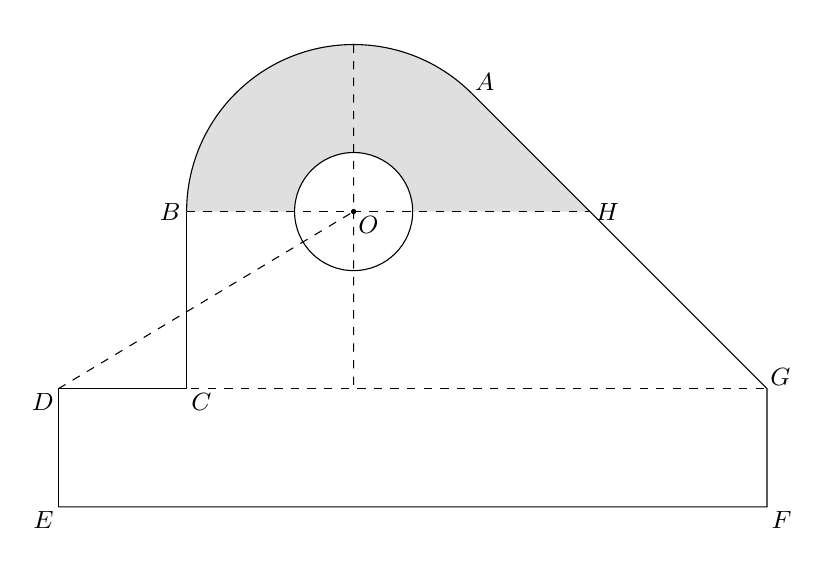
\begin{tikzpicture}[scale=0.75, font=\small]
  \coordinate (D) at (0,2);
  \coordinate (E) at (0,0);
  \coordinate (F) at (12,0);
  \coordinate (G) at (12,2);
  \coordinate (O) at (5,5);
  \coordinate (A) at (7,7);
  \coordinate (B) at (2.1716,5);
  \coordinate (C) at (2.1716,2);
  \coordinate (H) at (9,5);
  \coordinate (T) at (5,7.8284);
  % ---------- 阴影：弧 B→A + AH + HB，随后把圆孔填白 ----------
  \fill[gray!25] (B) arc[start angle=180, end angle=45, radius=2.8284] -- (H) -- cycle;
  \fill[white] (O) circle (1);
  % ---------- 虚线 ----------
  \draw[dashed] (B) -- (H);
  \draw[dashed] (D) -- (G);
  \draw[dashed] (T) -- (5,2);
  \draw[dashed] (D) -- (O);
  % ---------- 实线轮廓与圆孔 ----------
  \draw (E) -- (F) -- (G) -- (A);
  \draw (A) arc[start angle=45, end angle=180, radius=2.8284];
  \draw (B) -- (C) -- (D) -- (E);
  \draw (O) circle (1);
  \fill (O) circle (1.3pt);
  % ---------- 标签 ----------
  \node[above right, inner sep=1pt] at (A) {$A$};
  \node[left, inner sep=2pt] at (B) {$B$};
  \node[below right, inner sep=1.5pt] at (C) {$C$};
  \node[below left, inner sep=1.5pt] at (D) {$D$};
  \node[below left, inner sep=1.5pt] at (E) {$E$};
  \node[below right, inner sep=1.5pt] at (F) {$F$};
  \node[above right, inner sep=1pt] at (G) {$G$};
  \node[right, inner sep=2pt] at (H) {$H$};
  \node[below right, inner sep=1.5pt] at (O) {$O$};
\end{tikzpicture}
\end{center}

\textbf{解析}

\textbf{第一步，建立坐标系（本题的胜负手）。}

以 $E$ 为原点，$EF$ 所在直线为 $x$ 轴、$ED$ 所在直线为 $y$ 轴。由 $EF=12$、$DE=2$ 及 $DEFG$ 为矩形：

\[E(0,0),\quad F(12,0),\quad G(12,2),\quad D(0,2)\]

\textbf{$A$ 的坐标由题给的两个 $7$ 直接定死}：$A$ 到直线 $DE$（即 $y$ 轴）的距离为 $7$，到直线 $EF$（即 $x$ 轴）的距离也为 $7$：

\[A(7,7)\]

\textbf{第二步，用两个条件解出圆心 $O$。}

设 $O\left(x_0,y_0\right)$。

\textbf{条件 ①：$AG$ 与圆相切于 $A$，故 $OA\perp AG$。}

\[\overrightarrow{AG}=G-A=(12-7,\ 2-7)=(5,-5)\ \parallel\ (1,-1)\]

\[\overrightarrow{AO}\cdot(1,-1)=0\ \Longrightarrow\ \left(x_0-7\right)-\left(y_0-7\right)=0\ \Longrightarrow\ y_0=x_0\]

\textbf{条件 ②：$\tan\angle ODC=\dfrac35$。}

$C$ 在 $DG$ 上，而 $DG$ 是水平的（$D(0,2)$、$G(12,2)$），故 $\overrightarrow{DC}$ 沿 $x$ 轴正向。$\angle ODC$ 就是 $DO$ 与水平方向的夹角：

\[\tan\angle ODC=\frac{y_0-2}{x_0}=\frac35\]

\textbf{联立}（把 $y_0=x_0$ 代入）：

\[\frac{x_0-2}{x_0}=\frac35\ \Longrightarrow\ 5x_0-10=3x_0\ \Longrightarrow\ x_0=5\]

\[\boxed{O(5,5)}\]

\textbf{半径}：

\[R=|OA|=\sqrt{(7-5)^{2}+(7-5)^{2}}=2\sqrt2\]

\textbf{第三步，定出 $B$、$C$、$H$。}

\textbf{$B$}：圆弧与 $BC$ 相切于 $B$，故 $OB\perp BC$；而 $BC\perp DG$（水平）说明 $BC$ \textbf{竖直}，于是 $OB$ \textbf{水平}：

\[B\left(5-2\sqrt2,\ 5\right),\qquad C\left(5-2\sqrt2,\ 2\right),\qquad BC=5-2=3\]

\textbf{$H$}：$BH\parallel DG$ 即 $H$ 在直线 $y=5$ 上；同时 $H$ 在直线 $AG$ 上。$AG$ 上的点可写成 $(7+t,\ 7-t)$，令 $7-t=5$ 得 $t=2$：

\[H(9,5)\]

\textbf{关键结构}：$B$、$O$、$H$ 三点都在直线 $y=5$ 上，\textbf{三点共线}——这条直线正是阴影部分的下边界。

\textbf{第四步，分割求面积。}

阴影区域由 \textbf{弧 $BA$ + 线段 $AH$ + 线段 $HB$} 围成。以 $O$ 为分割中心，它恰好被 $OA$ 分成两块：

\textbf{① 扇形 $OBA$}

以 $O$ 为中心，$B$ 在正西方向（$180^\circ$），$A(7,7)$ 相对 $O$ 的方向是 $(2,2)$，即东北 $45^\circ$。弧从 $B$ 经最高点到 $A$，圆心角

\[180^\circ-45^\circ=135^\circ\]

\[S_1=\frac{135}{360}\pi R^{2}=\frac38\times\pi\times8=3\pi\]

\textbf{② 直角三角形 $OAH$}

因 $OA\perp AH$（切线性质），且

\[|OA|=2\sqrt2,\qquad |AH|=\sqrt{(9-7)^{2}+(5-7)^{2}}=2\sqrt2\]

\[S_2=\frac12\times2\sqrt2\times2\sqrt2=4\]

（顺带核对：$|OH|=\sqrt{|OA|^{2}+|AH|^{2}}=\sqrt{8+8}=4$，而由坐标 $|OH|=9-5=4$ ）

\textbf{③ 扣除圆孔}

圆孔的圆心恰是 $O$，而 $O$ \textbf{正落在阴影的下边界 $BH$ 上}。因此只有\textbf{上半个圆孔}位于阴影区域内：

\[S_3=\frac12\pi\times1^{2}=\frac\pi2\]

（半径 $1$ 远小于 $O$ 到两条边界的距离 $R=2\sqrt2\approx2.83$ 与 $|OA|=2\sqrt2$，故上半圆确实整个都在阴影内部。）

\textbf{第五步，合成。}

\[S=S_1+S_2-S_3=3\pi+4-\frac\pi2=4+\frac{5\pi}2\]

\textbf{答案：$4+\dfrac{5\pi}2$}（约 $11.85\ \mathrm{cm}^{2}$）

\begin{gktip}
\textbf{三个关键点}：
① \textbf{切点条件 = 半径垂直于切线}。本题两个切点各给一个垂直关系：$OA\perp AG$ 定出 $y_0=x_0$，$OB\perp BC$ 定出 $OB$ 水平（从而 $B$ 与 $O$ 等高）。
② \textbf{"$A$ 到两条边的距离均为 $7$"是把 $A$ 钉死在 $(7,7)$ 的唯一条件}，建系时必须以 $E$ 为原点才用得上它。
③ \textbf{圆孔只挖掉一半}——$O$ 在阴影的边界线上，多减 $\dfrac\pi2$ 或整个 $\pi$ 都是常见错误。\textbf{画完图先问一句：这个洞有多少落在阴影里？}

\textbf{分割策略}：任何"圆弧 + 直线"围成的区域，都优先尝试\textbf{从圆心向各顶点连线}，把它切成若干扇形与三角形。本题连一条 $OA$ 就切干净了。
\end{gktip}

\par\medskip

\gkpart{四、解答题（共 70 分）}

\gksolhead{17}{10 分}

\textbf{题目}　在① $ac=\sqrt3$，② $c\sin A=3$，③ $c=\sqrt3b$ 这三个条件中任选一个，补充在下面问题中，若问题中的三角形存在，求 $c$ 的值；若问题中的三角形不存在，说明理由。

问题：是否存在 $\triangle ABC$，它的内角 $A$，$B$，$C$ 的对边分别为 $a$，$b$，$c$，且 $\sin A=\sqrt3\sin B$，$C=\dfrac\pi6$，\gkblank{}？

\par\medskip

\textbf{第一步（三个选项共用）：把两个公共条件榨干。}

由\textbf{正弦定理}，$\sin A=\sqrt3\sin B$ 等价于

\[a=\sqrt3\,b\]

再由\textbf{余弦定理}，注意 $C=\dfrac\pi6$、$\cos C=\dfrac{\sqrt3}2$：

\[c^{2}=a^{2}+b^{2}-2ab\cos C=3b^{2}+b^{2}-2\cdot\sqrt3b\cdot b\cdot\frac{\sqrt3}2=4b^{2}-3b^{2}=b^{2}\]

因 $b,c>0$：

\[\boxed{c=b}\]

\textbf{这一步已经把三角形的形状完全定死了}：$b=c$ 说明 $\triangle ABC$ 是等腰三角形，$B=C=\dfrac\pi6$，从而

\[A=\pi-\frac\pi6-\frac\pi6=\frac{2\pi}3\]

三边之比恒为

\[a:b:c=\sqrt3:1:1\]

\textbf{校验}：$\sin A=\sin\dfrac{2\pi}3=\dfrac{\sqrt3}2$，而 $\sqrt3\sin B=\sqrt3\times\dfrac12=\dfrac{\sqrt3}2$ 

剩下的工作只是：用所选条件确定这个形状的\textbf{大小}（或判定它与已定形状冲突）。

\par\medskip

\textbf{选择条件 ①（$ac=\sqrt3$）}

由 $a=\sqrt3b=\sqrt3c$：

\[ac=\sqrt3c\cdot c=\sqrt3c^{2}=\sqrt3\ \Longrightarrow\ c^{2}=1\ \Longrightarrow\ c=1\]

\textbf{三角形存在}，此时 $a=\sqrt3$、$b=c=1$。

\textbf{验算}：$a^{2}=3$，$b^{2}+c^{2}-2bc\cos A=1+1-2\times\left(-\dfrac12\right)=3$ 

\[\boxed{c=1}\]

\par\medskip

\textbf{选择条件 ②（$c\sin A=3$）}

已求出 $A=\dfrac{2\pi}3$，$\sin A=\dfrac{\sqrt3}2$：

\[c\times\frac{\sqrt3}2=3\ \Longrightarrow\ c=\frac6{\sqrt3}=2\sqrt3\]

\textbf{三角形存在}，此时 $b=c=2\sqrt3$、$a=\sqrt3\times2\sqrt3=6$。

\textbf{验算}：$c\sin A=2\sqrt3\times\dfrac{\sqrt3}2=3$ 

\[\boxed{c=2\sqrt3}\]

\par\medskip

\textbf{选择条件 ③（$c=\sqrt3b$）}

由第一步已证 $c=b$。若同时要求 $c=\sqrt3b$，则

\[b=\sqrt3b\ \Longrightarrow\ \left(\sqrt3-1\right)b=0\ \Longrightarrow\ b=0\]

与三角形边长 $b>0$ 矛盾。

\textbf{所以满足条件 ③ 的三角形不存在。}

\textbf{另一角度的说明}（更直观）：条件 ③ 连同 $a=\sqrt3b$ 会给出 $a=c$，即 $A=C=\dfrac\pi6$；但由 $a=\sqrt3b$ 及正弦定理有 $\sin A=\sqrt3\sin B$，代入 $A=\dfrac\pi6$ 得 $\sin B=\dfrac1{2\sqrt3}$，于是 $B$ 不可能使三内角之和为 $\pi$（此时 $A+C=\dfrac\pi3$，要求 $B=\dfrac{2\pi}3$，但 $\sin\dfrac{2\pi}3=\dfrac{\sqrt3}2\ne\dfrac1{2\sqrt3}$）。矛盾同样成立。

\[\boxed{\text{不存在}}\]

\begin{gktip}
\textbf{方法总结（"结构不良"试题的通用打法）}：
\textbf{第一步永远是先把所有分支共有的条件用到极限}。本题的两个公共条件（$\sin A=\sqrt3\sin B$ 与 $C=\dfrac\pi6$）已经把三角形的\textbf{形状}唯一确定为 $a:b:c=\sqrt3:1:1$，三个待选条件各自只是一把"标尺"：
\begin{itemize}
\item ① 给出面积型的量 $ac$ → 定出大小；
\item ② 给出长度型的量 $c\sin A$（几何上就是 $B$ 到 $AC$ 的距离，即三角形的一条高）→ 定出大小；
\item ③ 给出的是\textbf{另一个比例关系}，与已经定死的比例冲突 → 无解。
\end{itemize}

\textbf{判定"不存在"的关键在于说清矛盾在哪}，只写"解不出来"不得分。本题的标准表述是"由公共条件已得 $b=c$，与 $c=\sqrt3b$ 矛盾"。
\end{gktip}

\par\medskip

\gksolhead{18}{12 分}

\textbf{题目}　已知公比大于 $1$ 的等比数列 $\left\{a_n\right\}$ 满足 $a_2+a_4=20$，$a_3=8$。

  (1) 求 $\left\{a_n\right\}$ 的通项公式；(2) 求 $a_1a_2-a_2a_3+\cdots+(-1)^{n-1}a_na_{n+1}$。

\par\medskip

\textbf{(1) 解}

设公比为 $q\ (q>1)$。\textbf{以 $a_3$ 为中心}表示相邻两项（这样只剩一个未知量）：

\[a_2=\frac{a_3}q=\frac8q,\qquad a_4=a_3q=8q\]

代入 $a_2+a_4=20$：

\[\frac8q+8q=20\]

两边乘 $q$（$q\ne0$）并整理：

\[8q^{2}-20q+8=0\ \Longrightarrow\ 2q^{2}-5q+2=0\ \Longrightarrow\ (2q-1)(q-2)=0\]

\[q=2\qquad\text{或}\qquad q=\frac12\]

由题设 $q>1$，\textbf{舍去} $q=\dfrac12$，得 $q=2$。

再由 $a_3=a_1q^{2}$：

\[a_1=\frac8{2^{2}}=2\]

\[a_n=2\times2^{\,n-1}=2^{\,n}\]

\textbf{检验}：$a_2+a_4=4+16=20$ ，$a_3=8$ 

\par\medskip

\textbf{(2) 解}

\textbf{第一步（关键）：先把 $a_na_{n+1}$ 算成一个新数列的通项。}

\[a_na_{n+1}=2^{\,n}\times2^{\,n+1}=2^{\,2n+1}=2\times4^{\,n}\]

于是待求的和是

\[S_n=\sum_{k=1}^{n}(-1)^{k-1}a_ka_{k+1}=\sum_{k=1}^{n}(-1)^{k-1}\cdot2\times4^{\,k}\]

\textbf{第二步：识别它本身就是等比数列求和。}

记第 $k$ 项为

\[b_k=(-1)^{k-1}\cdot2\times4^{\,k}\]

则

\[b_1=2\times4=8,\qquad \frac{b_{k+1}}{b_k}=\frac{(-1)^{k}\cdot2\times4^{\,k+1}}{(-1)^{k-1}\cdot2\times4^{\,k}}=-4\]

\textbf{$\left\{b_k\right\}$ 是首项 $8$、公比 $-4$ 的等比数列}，不必分奇偶讨论，直接套求和公式：

\[S_n=\frac{b_1\left[1-(-4)^{n}\right]}{1-(-4)}=\frac{8\left[1-(-4)^{n}\right]}5\]

\textbf{第三步，逐项验算。}

\begin{itemize}
\item $n=1$：$S_1=a_1a_2=2\times4=8$；公式给 $\dfrac{8(1+4)}5=8$ 
\item $n=2$：$S_2=8-a_2a_3=8-4\times8=-24$；公式给 $\dfrac{8(1-16)}5=-24$ 
\item $n=3$：$S_3=-24+a_3a_4=-24+8\times16=104$；公式给 $\dfrac{8(1+64)}5=104$ 
\end{itemize}

\[\boxed{S_n=\frac85\left[1-(-4)^{n}\right]}\]

也可写成

\[S_n=\frac{8+(-1)^{n-1}\cdot2^{\,2n+3}}5\]

\begin{gktip}
\textbf{方法总结}：形如 $\sum(-1)^{k-1}c_k$ 的交错和，\textbf{先算出 $c_k$ 的显式表达式}再判断结构，是唯一稳妥的路线。本题算完 $a_ka_{k+1}=2\cdot4^{k}$ 后会发现，\textbf{带上符号后它自己就是公比为 $-4$ 的等比数列}——直接套公式即可，完全不需要"分 $n$ 为奇数、偶数两种情形"的繁琐讨论（那是本题最常见的低效解法）。

\textbf{验算纪律}：数列求和的答案\textbf{必须用 $n=1,2,3$ 回代检验}。含 $(-4)^{n}$ 这类交错项时符号最容易写反，回代一次即可暴露。
\end{gktip}

\par\medskip

\gksolhead{19}{12 分}

\textbf{题目}　为加强环境保护，治理空气污染，环境监测部门对某市空气质量进行调研，随机抽查了 $100$ 天空气中的 PM2.5 和 $\mathrm{SO_2}$ 浓度（单位：$\mu\mathrm g/\mathrm m^{3}$），得下表：

\begin{center}
\begin{tabular}{cccc}
\toprule
$\mathrm{SO_2}$ 浓度 & $[0,50]$ & $(50,150]$ & $(150,475]$ \\
\midrule
PM2.5 $[0,35]$ & $32$ & $18$ & $4$ \\
PM2.5 $(35,75]$ & $6$ & $8$ & $12$ \\
PM2.5 $(75,115]$ & $3$ & $7$ & $10$ \\
\bottomrule
\end{tabular}
\end{center}

  (1) 估计"PM2.5 浓度不超过 $75$ 且 $\mathrm{SO_2}$ 浓度不超过 $150$"的概率；(2) 完成 $2\times2$ 列联表；(3) 判断是否有 $99\%$ 的把握认为两者有关。

\par\medskip

\textbf{(1) 解}

"PM2.5 浓度不超过 $75$"对应表中的\textbf{前两行}（$[0,35]$ 与 $(35,75]$）；"$\mathrm{SO_2}$ 浓度不超过 $150$"对应\textbf{前两列}（$[0,50]$ 与 $(50,150]$）。

把这 $2\times2$ 个格子相加：

\[32+18+6+8=64\]

用频率估计概率：

\[P=\frac{64}{100}=0.64\]

\gkanswer{答案：$0.64$}

\par\medskip

\textbf{(2) 解}

按"PM2.5 是否超过 $75$""$\mathrm{SO_2}$ 是否超过 $150$"两个二分标准合并原表：

\begin{itemize}
\item $[0,75]$ 且 $[0,150]$：$32+18+6+8=64$
\item $[0,75]$ 且 $(150,475]$：$4+12=16$
\item $(75,115]$ 且 $[0,150]$：$3+7=10$
\item $(75,115]$ 且 $(150,475]$：$10$
\end{itemize}

\textbf{$2\times2$ 列联表}

\begin{center}
\begin{tabular}{cccc}
\toprule
$\mathrm{SO_2}$ 浓度 & $[0,150]$ & $(150,475]$ & 合计 \\
\midrule
PM2.5 $[0,75]$ & $64$ & $16$ & $80$ \\
PM2.5 $(75,115]$ & $10$ & $10$ & $20$ \\
合计 & $74$ & $26$ & $100$ \\
\bottomrule
\end{tabular}
\end{center}

\textbf{校验}：$64+16+10+10=100$ （与抽查天数一致）

\par\medskip

\textbf{(3) 解}

\textbf{零假设 $H_0$}：该市一天空气中 PM2.5 浓度与 $\mathrm{SO_2}$ 浓度\textbf{无关}。

按列联表取 $a=64$、$b=16$、$c=10$、$d=10$，$n=100$。

\textbf{先算分子中的核心因子}：

\[ad-bc=64\times10-16\times10=640-160=480\]

\textbf{代入公式}：

\[K^{2}=\frac{n(ad-bc)^{2}}{(a+b)(c+d)(a+c)(b+d)}=\frac{100\times480^{2}}{80\times20\times74\times26}\]

\textbf{分子}：$100\times230400=23\,040\,000$

\textbf{分母}：$80\times20=1600$，$74\times26=1924$，$1600\times1924=3\,078\,400$

\[K^{2}=\frac{23\,040\,000}{3\,078\,400}\approx7.484\]

\textbf{与临界值比较}：

\[K^{2}\approx7.484>6.635=k_{0.010}\]

\textbf{结论}：能够拒绝零假设，即\textbf{有 $99\%$ 的把握认为该市一天空气中 PM2.5 浓度与 $\mathrm{SO_2}$ 浓度有关}。

\begin{gktip}
\textbf{书写规范}：独立性检验的完整作答必须包含四要素——① 提出零假设 $H_0$；② 代入公式算出 $K^{2}$；③ 与临界值 $6.635$ 比较；④ 用"有关/无关"下结论。缺任何一步都要扣分。

\textbf{合并列联表时最容易出错的地方}：$(35,75]$ 这一行属于"$[0,75]$"（要并进第一行），而 $(50,150]$ 这一列属于"$[0,150]$"（要并进第一列）。\textbf{先把原表的行列分组画出来再加，比直接心算可靠得多。}

\textbf{数值自检}：算完 $K^{2}$ 后回看列联表——第一行 $64:16=4:1$、第二行 $10:10=1:1$，两行的比例差别明显，与"有关"的结论方向一致。若算出的 $K^{2}$ 很小却看到比例相差悬殊，一定是算错了。
\end{gktip}

\par\medskip

\gksolhead{20}{12 分}

\textbf{题目}　如图，四棱锥 $P\text{-}ABCD$ 的底面为正方形，$PD\perp$ 底面 $ABCD$。设平面 $PAD$ 与平面 $PBC$ 的交线为 $l$。

\begin{center}% 2020 新高考Ⅱ卷 20：四棱锥 P-ABCD（底面 ABCD 为正方形，PD⊥底面 ABCD）
% 绘制依据：源 PDF 原图。底面按斜二测画：A 左前、B 右前、C 右后、D 中后（被遮挡顶点）；
% PD 垂直底面，故 P 画在 D 的正上方（位于版面中偏左）。
% 实线：PA、PB、PC、AB、BC；虚线：PD、AD、DC。只标 P、A、B、C、D 五点。
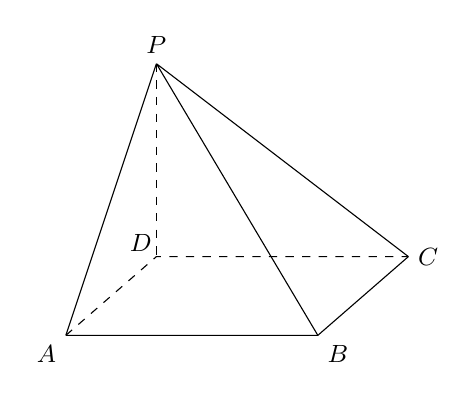
\begin{tikzpicture}[scale=1.0, font=\small]
  \coordinate (A) at (0,0);
  \coordinate (B) at (3.2,0);
  \coordinate (C) at (4.35,1.0);
  \coordinate (D) at (1.15,1.0);
  \coordinate (P) at (1.15,3.45);
  \draw (P) -- (A)  (P) -- (B)  (P) -- (C);
  \draw (A) -- (B) -- (C);
  \draw[dashed] (P) -- (D);
  \draw[dashed] (A) -- (D) -- (C);
  \node[above] at (P) {$P$};
  \node[below left] at (A) {$A$};
  \node[below right] at (B) {$B$};
  \node[right] at (C) {$C$};
  \node[above left, inner sep=1.5pt] at (D) {$D$};
\end{tikzpicture}
\end{center}

  (1) 证明：$l\perp$ 平面 $PDC$；(2) 已知 $PD=AD=1$，$Q$ 为 $l$ 上的点，$QB=\sqrt2$，求 $PB$ 与平面 $QCD$ 所成角的正弦值。

\par\medskip

\textbf{(1) 证明}

\textbf{第一步，先弄清交线 $l$ 的方向（本问的关键）。}

底面是正方形，故 $BC\parallel AD$。

又 $AD\subset$ 平面 $PAD$，$BC\not\subset$ 平面 $PAD$，由\textbf{线面平行的判定定理}：

\[BC\parallel\text{平面 }PAD\]

而 $BC\subset$ 平面 $PBC$，且

\[\text{平面 }PBC\cap\text{平面 }PAD=l\]

由\textbf{线面平行的性质定理}（过该直线的平面与已知平面的交线平行于该直线）：

\[BC\parallel l\]

\textbf{第二步，证明 $BC\perp$ 平面 $PDC$。}

\begin{itemize}
\item $PD\perp$ 底面 $ABCD$，而 $BC\subset$ 底面 $ABCD$，故 $PD\perp BC$；
\item 底面是\textbf{正方形}，故 $BC\perp CD$；
\item $PD\cap CD=D$，且 $PD$、$CD$ 都在平面 $PDC$ 内。
\end{itemize}

由\textbf{线面垂直的判定定理}：

\[BC\perp\text{平面 }PDC\]

\textbf{第三步，平移过去。}

由 $l\parallel BC$ 及"两平行线中一条垂直于某平面，则另一条也垂直于该平面"：

\[l\perp\text{平面 }PDC\qquad\blacksquare\]

\par\medskip

\textbf{(2) 解}

\textbf{建系}：由 $PD\perp$ 底面且底面为正方形，以 $D$ 为原点，$DA$、$DC$、$DP$ 三条两两垂直的棱为 $x$、$y$、$z$ 轴。

由 $PD=AD=1$（正方形边长为 $1$）：

\[D(0,0,0),\quad A(1,0,0),\quad B(1,1,0),\quad C(0,1,0),\quad P(0,0,1)\]

\textbf{写出 $l$ 的参数形式}：由 (1) 知 $l\parallel BC$，而 $\overrightarrow{BC}=(-1,0,0)$ 即沿 $x$ 轴方向；又 $l$ 过点 $P$（两平面的公共点）。故

\[l:\ (t,\ 0,\ 1),\qquad t\in\mathbf R\]

\textbf{用 $QB=\sqrt2$ 定出 $Q$}：设 $Q(t,0,1)$，

\[|QB|^{2}=(t-1)^{2}+(0-1)^{2}+(1-0)^{2}=(t-1)^{2}+2\]

令其等于 $\left(\sqrt2\right)^{2}=2$：

\[(t-1)^{2}=0\ \Longrightarrow\ t=1\]

\[Q(1,0,1)\]

（$Q$ 恰在 $A$ 的正上方，即 $Q$ 与 $P$、$A$、$D$ 构成正方形 $PDAQ$。）

\textbf{求平面 $QCD$ 的法向量}：平面过 $D(0,0,0)$，

\[\overrightarrow{DC}=(0,1,0),\qquad \overrightarrow{DQ}=(1,0,1)\]

\[\boldsymbol n=\overrightarrow{DC}\times\overrightarrow{DQ}=\begin{vmatrix}\boldsymbol i&\boldsymbol j&\boldsymbol k\\0&1&0\\1&0&1\end{vmatrix}=(1\times1-0\times0,\ \ 0\times1-0\times1,\ \ 0\times0-1\times1)=(1,\ 0,\ -1)\]

\textbf{验证}：$\boldsymbol n\cdot\overrightarrow{DC}=0$ ，$\boldsymbol n\cdot\overrightarrow{DQ}=1-1=0$ 

\textbf{求线面角}：

\[\overrightarrow{PB}=B-P=(1,1,-1),\qquad \left|\overrightarrow{PB}\right|=\sqrt3,\qquad |\boldsymbol n|=\sqrt2\]

\[\overrightarrow{PB}\cdot\boldsymbol n=1\times1+1\times0+(-1)\times(-1)=2\]

设所求角为 $\theta$。\textbf{线面角的正弦等于方向向量与法向量夹角的余弦的绝对值}：

\[\sin\theta=\frac{\left|\overrightarrow{PB}\cdot\boldsymbol n\right|}{\left|\overrightarrow{PB}\right||\boldsymbol n|}=\frac2{\sqrt3\times\sqrt2}=\frac2{\sqrt6}=\frac{\sqrt6}3\]

\textbf{所以 $PB$ 与平面 $QCD$ 所成角的正弦值为 $\dfrac{\sqrt6}3$。}

（核对：$\dfrac{\sqrt6}3\approx0.816<1$，是合法的正弦值。）

\begin{gktip}
\textbf{方法总结}：
① \textbf{第 (1) 问是第 (2) 问的"许可证"}——只有先证出 $l\parallel BC$，才能在建系后写出 $l$ 的参数方程。\textbf{解答题里前一问的结论几乎总是后一问要用的工具，不要跳过。}
② \textbf{$QB=\sqrt2$ 这个条件其实卡在最小值上}：$|QB|^{2}=(t-1)^{2}+2\ge2$，最小值 $\sqrt2$ 恰在 $t=1$ 取到。因此方程解出\textbf{重根}是正常现象，不是算错。遇到"距离恰为某个值"而方程出现重根时，先想一想是不是命题人故意让它唯一。
③ \textbf{线面角公式最容易记混}：用法向量算出来的是\textbf{正弦}（不是余弦），因为法向量与直线的夹角是所求角的余角。写成 $\sin\theta=\left|\cos\left\langle\text{\text{方向向量}},\ \text{\text{法向量}}\right\rangle\right|$ 就不会错。
\end{gktip}

\par\medskip

\gksolhead{21}{12 分}

\textbf{题目}　已知椭圆 $C:\dfrac{x^{2}}{a^{2}}+\dfrac{y^{2}}{b^{2}}=1\ (a>b>0)$ 过点 $M(2,3)$，点 $A$ 为其左顶点，且 $AM$ 的斜率为 $\dfrac12$。

  (1) 求 $C$ 方程；(2) 点 $N$ 为椭圆上任意一点，求 $\triangle AMN$ 的面积的最大值。

\par\medskip

\textbf{(1) 解}

\textbf{第一步，用斜率条件求 $a$。}

左顶点为 $A(-a,0)$。由 $AM$ 的斜率为 $\dfrac12$：

\[k_{AM}=\frac{3-0}{2-(-a)}=\frac3{2+a}=\frac12\]

\[2+a=6\ \Longrightarrow\ a=4\]

\textbf{第二步，用"$M$ 在椭圆上"求 $b^{2}$。}

把 $M(2,3)$、$a^{2}=16$ 代入：

\[\frac{2^{2}}{16}+\frac{3^{2}}{b^{2}}=1\ \Longrightarrow\ \frac14+\frac9{b^{2}}=1\ \Longrightarrow\ \frac9{b^{2}}=\frac34\ \Longrightarrow\ b^{2}=12\]

\textbf{检验} $a>b>0$：$16>12>0$ 

\[\boxed{C:\ \frac{x^{2}}{16}+\frac{y^{2}}{12}=1}\]

（此时 $A(-4,0)$，代入验证 $\dfrac{16}{16}+0=1$ ）

\par\medskip

\textbf{(2) 解}

\textbf{思路}：$A$、$M$ 是\textbf{定点}，所以 $|AM|$ 是\textbf{定长}（"定弦"）；面积

\[S=\frac12|AM|\cdot d(N,\ AM)\]

只随 $N$ 到直线 $AM$ 的距离变化。于是问题化为：\textbf{求椭圆上的点到定直线 $AM$ 的最大距离。}

\textbf{第一步，算定弦长与定直线方程。}

\[|AM|=\sqrt{\left[2-(-4)\right]^{2}+(3-0)^{2}}=\sqrt{36+9}=\sqrt{45}=3\sqrt5\]

直线 $AM$：过 $A(-4,0)$、斜率 $\dfrac12$：

\[y=\frac12(x+4)\ \Longrightarrow\ x-2y+4=0\]

\textbf{第二步，用参数方程求最大距离。}

设椭圆上的点

\[N\left(4\cos\theta,\ 2\sqrt3\sin\theta\right)\]

\[d=\frac{\left|4\cos\theta-2\times2\sqrt3\sin\theta+4\right|}{\sqrt{1^{2}+(-2)^{2}}}=\frac{\left|4\cos\theta-4\sqrt3\sin\theta+4\right|}{\sqrt5}\]

\textbf{辅助角公式}（把 $4\cos\theta-4\sqrt3\sin\theta$ 合成一项）：振幅为 $\sqrt{4^{2}+\left(4\sqrt3\right)^{2}}=\sqrt{16+48}=8$，

\[4\cos\theta-4\sqrt3\sin\theta=8\left(\frac12\cos\theta-\frac{\sqrt3}2\sin\theta\right)=8\cos\left(\theta+\frac\pi3\right)\]

\[d=\frac{\left|8\cos\left(\theta+\dfrac\pi3\right)+4\right|}{\sqrt5}\]

因 $\cos\left(\theta+\dfrac\pi3\right)\in[-1,1]$，括号内的值域为 $[-4,12]$，绝对值的最大值为

\[d_{\max}=\frac{12}{\sqrt5}=\frac{12\sqrt5}5\]

在 $\cos\left(\theta+\dfrac\pi3\right)=1$ 即 $\theta=-\dfrac\pi3$ 时取到，对应

\[N\left(4\cos\left(-\frac\pi3\right),\ 2\sqrt3\sin\left(-\frac\pi3\right)\right)=(2,\ -3)\]

\textbf{恰好是 $M(2,3)$ 关于 $x$ 轴的对称点}。

\textbf{第三步，求面积。}

\[S_{\max}=\frac12\times3\sqrt5\times\frac{12}{\sqrt5}=\frac12\times36=18\]

\[\boxed{S_{\max}=18}\]

\par\medskip

\textbf{第二种解法（平移切线法，可作验算）}

把直线 $x-2y+4=0$ 平行移动为 $x-2y+m=0$，当它与椭圆\textbf{相切}时，切点就是距离最远（或最近）的点。

由 $x=2y-m$ 代入 $3x^{2}+4y^{2}=48$（即 $\dfrac{x^{2}}{16}+\dfrac{y^{2}}{12}=1$ 去分母）：

\[3(2y-m)^{2}+4y^{2}=48\ \Longrightarrow\ 16y^{2}-12my+3m^{2}-48=0\]

相切要求判别式为零：

\[\Delta=144m^{2}-64\left(3m^{2}-48\right)=-48m^{2}+3072=0\ \Longrightarrow\ m^{2}=64\ \Longrightarrow\ m=\pm8\]

两条切线为 $x-2y+8=0$ 与 $x-2y-8=0$，它们到 $AM$（$m=4$）的距离分别是

\[\frac{|8-4|}{\sqrt5}=\frac4{\sqrt5},\qquad \frac{|-8-4|}{\sqrt5}=\frac{12}{\sqrt5}\]

取较大者 $\dfrac{12}{\sqrt5}$  与解法一一致。

切点：把 $m=-8$ 代回 $16y^{2}+96y+144=0$ 得 $y=-3$，$x=2(-3)+8=2$，即 $N(2,-3)$ 

\begin{gktip}
\textbf{方法总结}：\textbf{"定弦 + 动点"型面积最值，一律拆成 $S=\dfrac12\times(\text{\text{定弦长}})\times(\text{\text{最大距离}})$}，把二元最值问题降为一元。

求"圆锥曲线上的点到定直线的最大距离"有两条通法：
① \textbf{参数方程 + 辅助角公式}（本题解法一）——机械、不易漏解，推荐作为主解法；
② \textbf{平移直线至相切}（解法二）——几何意义清晰，且能顺带求出切点，最适合用来验算。

\textbf{两法互验是这类题最可靠的做法}：解法一容易在辅助角的振幅上算错，解法二容易在判别式上算错，两者独立，同时出错的概率很低。
\end{gktip}

\par\medskip

\gksolhead{22}{12 分}

\textbf{题目}　已知函数 $f(x)=a\mathrm e^{x-1}-\ln x+\ln a$。

  (1) 当 $a=\mathrm e$ 时，求曲线 $y=f(x)$ 在点 $(1,f(1))$ 处的切线与两坐标轴围成的三角形的面积；(2) 若 $f(x)\ge1$，求 $a$ 的取值范围。

\par\medskip

\textbf{(1) 解}

\textbf{第一步，把 $a=\mathrm e$ 代入并化简。}

\[f(x)=\mathrm e\cdot\mathrm e^{x-1}-\ln x+\ln\mathrm e=\mathrm e^{x}-\ln x+1\]

\textbf{第二步，求切点与斜率。}

\[f(1)=\mathrm e^{1}-\ln1+1=\mathrm e+1\]

\[f'(x)=\mathrm e^{x}-\frac1x\ \Longrightarrow\ f'(1)=\mathrm e-1\]

\textbf{第三步，写切线方程。}

\[y-(\mathrm e+1)=(\mathrm e-1)(x-1)\]

\[y=(\mathrm e-1)x-(\mathrm e-1)+\mathrm e+1=(\mathrm e-1)x+2\]

\textbf{第四步，求两个截距并算面积。}

\begin{itemize}
\item 令 $x=0$：$y=2$，纵截距 $2$；
\item 令 $y=0$：$x=-\dfrac2{\mathrm e-1}$，横截距的绝对值为 $\dfrac2{\mathrm e-1}$。
\end{itemize}

\[S=\frac12\times\frac2{\mathrm e-1}\times2=\frac2{\mathrm e-1}\]

\[\boxed{S=\frac2{\mathrm e-1}}\]

（数值核对：$\mathrm e-1\approx1.718$，$S\approx1.164$。）

\par\medskip

\textbf{(2) 解}

\textbf{定义域}：$\ln x$ 要求 $x>0$；$\ln a$ 要求 $a>0$。

\textbf{第一步（本题的钥匙）：把不等式化成"同一个函数在两点的比较"。}

利用 $a\mathrm e^{x-1}=\mathrm e^{x-1+\ln a}$ 与 $x=\mathrm e^{\ln x}$，构造函数

\[g(t)=\mathrm e^{t}+t\]

计算

\[g\left(x-1+\ln a\right)=\mathrm e^{\,x-1+\ln a}+\left(x-1+\ln a\right)=a\mathrm e^{x-1}+x-1+\ln a\]

\[g(\ln x)=\mathrm e^{\ln x}+\ln x=x+\ln x\]

两式相减：

\[g\left(x-1+\ln a\right)-g(\ln x)=a\mathrm e^{x-1}+\ln a-\ln x-1=f(x)-1\]

于是得到恒等式

\[\boxed{f(x)-1=g\left(x-1+\ln a\right)-g(\ln x)}\]

\textbf{第二步，用 $g$ 的单调性脱去 $g$。}

\[g'(t)=\mathrm e^{t}+1>0\]

$g$ 在 $\mathbf R$ 上\textbf{严格递增}，因此

\[f(x)\ge1\ \Longleftrightarrow\ g\left(x-1+\ln a\right)\ge g(\ln x)\ \Longleftrightarrow\ x-1+\ln a\ge\ln x\]

\textbf{第三步，分离参数求最值。}

上式对一切 $x>0$ 成立，等价于

\[\ln a\ge\ln x-x+1\qquad\text{对一切 }x>0\]

即 $\ln a$ 不小于右边的\textbf{最大值}。令

\[h(x)=\ln x-x+1\qquad(x>0)\]

\[h'(x)=\frac1x-1=\frac{1-x}x\]

\begin{center}
\begin{tabular}{cccc}
\toprule
$x$ & $(0,1)$ & $1$ & $(1,+\infty)$ \\
\midrule
$h'(x)$ & $+$ & $0$ & $-$ \\
$h(x)$ & 增 & 极大 & 减 \\
\bottomrule
\end{tabular}
\end{center}

\[h_{\max}=h(1)=\ln1-1+1=0\]

（这正是著名的不等式 $\ln x\le x-1$。）

\textbf{第四步，得出结论。}

\[\ln a\ge0\ \Longrightarrow\ a\ge1\]

\[\boxed{a\in[1,+\infty)}\]

\textbf{验证端点 $a=1$}：此时 $f(x)=\mathrm e^{x-1}-\ln x$，

\[f'(x)=\mathrm e^{x-1}-\frac1x\]

$f'(1)=1-1=0$，且 $f'$ 在 $(0,1)$ 为负、在 $(1,+\infty)$ 为正，故 $x=1$ 是最小值点：

\[f(1)=\mathrm e^{0}-\ln1=1\ge1\quad\checkmark\]

恰好取到等号，说明 $a=1$ \textbf{必须包含在答案里}。

\textbf{验证 $a<1$ 不行}：取 $a=0.9$，$f(1)=0.9\mathrm e^{0}-0+\ln0.9=0.9-0.105=0.795<1$ 

\par\medskip

\begin{gktip}
\textbf{方法总结（本题的三个层次）}：

1. \textbf{同构是本题的核心技巧}。$a\mathrm e^{x-1}$ 里的 $a$ 藏在系数位置，直接求导会得到 $f'(x)=a\mathrm e^{x-1}-\dfrac1x$，其零点 $x_0$ 无法用初等函数表示，讨论起来非常麻烦。而把 $a$ \textbf{搬进指数}（$a\mathrm e^{x-1}=\mathrm e^{x-1+\ln a}$）、把 $x$ \textbf{写成 $\mathrm e^{\ln x}$}，两边就变成同一个函数 $g(t)=\mathrm e^{t}+t$ 在两个自变量处的取值，一步脱去。

2. \textbf{识别同构的信号}：式子里同时出现 $\mathrm e^{(\cdot)}$ 与 $\ln(\cdot)$、且它们的"配对量"能凑成 $\mathrm e^{u}+u$ 或 $u\mathrm e^{u}$ 的形式时，几乎一定是同构题。\textbf{常用的三个母函数是 $g(t)=\mathrm e^{t}+t$、$g(t)=t\mathrm e^{t}$、$g(t)=\dfrac{\mathrm e^{t}}t$。}

3. \textbf{$\ln x\le x-1$ 是必备工具}。第三步中 $h(x)=\ln x-x+1$ 的最大值为 $0$，正是这条基本不等式；见到 $\ln x-x$ 的组合应当条件反射地想到它，可以省去求导过程。

\textbf{考试策略}：第 (1) 问是送分题（求导 + 写切线 + 算截距），必须拿满；第 (2) 问若想不到同构，退而求其次的做法是设 $f'(x_0)=0$、用 $a\mathrm e^{x_0-1}=\dfrac1{x_0}$ 把最小值 $f\left(x_0\right)$ 表示出来再讨论——过程长得多，但仍可得分。\textbf{压轴题不要因为看不出巧解就放弃，先把能写的写上。}
\end{gktip}
